\protect \hypertarget {soln:1.1}{}
\begin{solution}{{1.1}}
  $\P(X=1)=3/5$, $\P(X=2)=3/10$, $\P(X=3)=1/10$, $\E(X)=1.5$
\end{solution}
\protect \hypertarget {soln:1.2}{}
\begin{solution}{{1.2}}
\end{solution}
\protect \hypertarget {soln:1.3}{}
\begin{solution}{{1.3}}
\end{solution}
\protect \hypertarget {soln:1.4}{}
\begin{solution}{{1.4}}
   N 3 4 5

  2/8 3/8 3/8
\end{solution}
\protect \hypertarget {soln:1.5}{}
\begin{solution}{{1.5}}
\end{solution}
\protect \hypertarget {soln:1.6}{}
\begin{solution}{{1.6}}
  5/11 и 6/11
\end{solution}
\protect \hypertarget {soln:1.7}{}
\begin{solution}{{1.7}}
  N — количество подбрасываний, G — количество орлов, R — решек

  E(N)=10/7, E(G)=1, E(R)=10/7-1=3/7
\end{solution}
\protect \hypertarget {soln:1.8}{}
\begin{solution}{{1.8}}
\end{solution}
\protect \hypertarget {soln:1.9}{}
\begin{solution}{{1.9}}
  у Саши 3/4
\end{solution}
\protect \hypertarget {soln:1.10}{}
\begin{solution}{{1.10}}
  стоп на 4-5-6 или стоп на 5-6
\end{solution}
\protect \hypertarget {soln:1.11}{}
\begin{solution}{{1.11}}
  $\P(X=4)=1/8$, $\E(X)=3$
\end{solution}
\protect \hypertarget {soln:1.12}{}
\begin{solution}{{1.12}}
\end{solution}
\protect \hypertarget {soln:2.1}{}
\begin{solution}{{2.1}}
\end{solution}
\protect \hypertarget {soln:2.2}{}
\begin{solution}{{2.2}}
\end{solution}
\protect \hypertarget {soln:2.3}{}
\begin{solution}{{2.3}}
\end{solution}
\protect \hypertarget {soln:2.4}{}
\begin{solution}{{2.4}}
\end{solution}
\protect \hypertarget {soln:2.5}{}
\begin{solution}{{2.5}}
\end{solution}
\protect \hypertarget {soln:2.6}{}
\begin{solution}{{2.6}}
  1/2
\end{solution}
\protect \hypertarget {soln:2.7}{}
\begin{solution}{{2.7}}
  $\E(X)=0.25\cdot 2 + 0.5\cdot (\E(X)+1)+0.25\cdot (\E(X)+2)$

  $\E(Y)=0.25\cdot 0 + 0.5\cdot (\E(Y)+1)+0.25\cdot (\E(Y)+1)$
\end{solution}
\protect \hypertarget {soln:2.8}{}
\begin{solution}{{2.8}}
стратегия 1: говорить стоп, если на кону 200 рублей вне зависимости от числа набранных красных карточек

 стратегия 2: если нет красных карточек или одна, то останавливаться при 200 рублях, а при двух карточках останавливаться на 100 рублях.
\end{solution}
\protect \hypertarget {soln:2.9}{}
\begin{solution}{{2.9}}
\end{solution}
\protect \hypertarget {soln:2.10}{}
\begin{solution}{{2.10}}
\end{solution}
\protect \hypertarget {soln:2.11}{}
\begin{solution}{{2.11}}
\end{solution}
\protect \hypertarget {soln:2.12}{}
\begin{solution}{{2.12}}
\end{solution}
\protect \hypertarget {soln:2.13}{}
\begin{solution}{{2.13}}
\end{solution}
\protect \hypertarget {soln:2.14}{}
\begin{solution}{{2.14}}
\end{solution}
\protect \hypertarget {soln:2.15}{}
\begin{solution}{{2.15}}
\end{solution}
\protect \hypertarget {soln:2.16}{}
\begin{solution}{{2.16}}
\end{solution}
\protect \hypertarget {soln:3.1}{}
\begin{solution}{{3.1}}
  $\P(A\mid B)=\frac{\P(A \cap B)}{\P(B)}= \frac{1/3}{1/6+1/3}=2/3$
\end{solution}
\protect \hypertarget {soln:3.2}{}
\begin{solution}{{3.2}}
  $A$ -- первый охотник попал в утку, $B$ — в утку попала ровно одна пуля

  $\P(A \mid B)=\frac{\P(A \cap B)}{\P(B)}= \frac{0.4 \cdot 0.3 }{0.4\cdot 0.3 + 0.6\cdot 0.7}=2/9$
\end{solution}
\protect \hypertarget {soln:3.3}{}
\begin{solution}{{3.3}}
  $\P(A \mid B)=1/6$
\end{solution}
\protect \hypertarget {soln:3.4}{}
\begin{solution}{{3.4}}
\[
\P(X = 2) = \frac{C_4^2 C_{48}^{11}}{C_{52}^{13}}
\]
$\P(X\geq 2 \mid X\geq 1)=\frac{\P(X \geq 2)}{\P(X \geq 1)}= \approx 0.37$
\end{solution}
\protect \hypertarget {soln:3.5}{}
\begin{solution}{{3.5}}
  $\P(A \mid B)=\frac{\P(A \cap B)}{\P(B)}= \frac{7\cdot 11 /C_{7+5+11}^2}{(7\cdot 11+5\cdot 11 + 7\cdot 5) /C_{7+5+11}^2 }$
\end{solution}
\protect \hypertarget {soln:3.6}{}
\begin{solution}{{3.6}}
  $B$ — событие, второй — черный, $\P(B)=11/16$

  $\P(A \mid B)=\P(A \cap B)/\P(B)=\frac{\frac{5}{16}\frac{11}{15}}{11/16}$
\end{solution}
\protect \hypertarget {soln:3.7}{}
\begin{solution}{{3.7}}
  $A$ — партия мяса заражена, $B$ — партия мяса по тесту заражена

  $\P(A \mid B)=\P(A \cap B)/\P(B)=\frac{0.04\cdot 0.9}{0.04\cdot 0.9+0.96\cdot 0.1}\approx 0.27$
\end{solution}
\protect \hypertarget {soln:3.8}{}
\begin{solution}{{3.8}}
  $A$ — Петя из Б класса, $B$ — Петя обожает географию

  $\P(A \mid B)=\P(A \cap B)/\P(B)=\frac{0.4/3}{0.3/3+0.4/3+0.7/3}=2/7$
\end{solution}
\protect \hypertarget {soln:3.9}{}
\begin{solution}{{3.9}}
  $1/3$
\end{solution}
\protect \hypertarget {soln:3.10}{}
\begin{solution}{{3.10}}
  да
\end{solution}
\protect \hypertarget {soln:3.11}{}
\begin{solution}{{3.11}}
  нет, $(4/52)\cdot (3/51)=\P(A\cap B) \neq \P(A)\cdot \P(B)=(4/52)^2$
\end{solution}
\protect \hypertarget {soln:3.12}{}
\begin{solution}{{3.12}}
\end{solution}
\protect \hypertarget {soln:3.13}{}
\begin{solution}{{3.13}}
$ 2/3 $, $1/2$, $ 1/2 $, $ 14/27 $
\end{solution}
\protect \hypertarget {soln:4.1}{}
\begin{solution}{{4.1}}
\end{solution}
\protect \hypertarget {soln:4.2}{}
\begin{solution}{{4.2}}
\end{solution}
\protect \hypertarget {soln:4.3}{}
\begin{solution}{{4.3}}
\end{solution}
\protect \hypertarget {soln:4.4}{}
\begin{solution}{{4.4}}
\end{solution}
\protect \hypertarget {soln:4.5}{}
\begin{solution}{{4.5}}
\end{solution}
\protect \hypertarget {soln:5.1}{}
\begin{solution}{{5.1}}
\end{solution}
\protect \hypertarget {soln:5.2}{}
\begin{solution}{{5.2}}
\end{solution}
\protect \hypertarget {soln:5.3}{}
\begin{solution}{{5.3}}
\end{solution}
\protect \hypertarget {soln:5.4}{}
\begin{solution}{{5.4}}
\end{solution}
\protect \hypertarget {soln:5.5}{}
\begin{solution}{{5.5}}
\end{solution}
\protect \hypertarget {soln:5.6}{}
\begin{solution}{{5.6}}
\end{solution}
\protect \hypertarget {soln:5.7}{}
\begin{solution}{{5.7}}
\end{solution}
\protect \hypertarget {soln:5.8}{}
\begin{solution}{{5.8}}
\end{solution}
\protect \hypertarget {soln:5.9}{}
\begin{solution}{{5.9}}
\end{solution}
\protect \hypertarget {soln:5.10}{}
\begin{solution}{{5.10}}
\end{solution}
\protect \hypertarget {soln:5.11}{}
\begin{solution}{{5.11}}
\end{solution}
\protect \hypertarget {soln:5.12}{}
\begin{solution}{{5.12}}
при $c=1/\E(X)$
\end{solution}
\protect \hypertarget {soln:5.13}{}
\begin{solution}{{5.13}}
\end{solution}
\protect \hypertarget {soln:5.14}{}
\begin{solution}{{5.14}}
\end{solution}
\protect \hypertarget {soln:5.15}{}
\begin{solution}{{5.15}}
\end{solution}
\protect \hypertarget {soln:5.16}{}
\begin{solution}{{5.16}}
\end{solution}
\protect \hypertarget {soln:6.1}{}
\begin{solution}{{6.1}}

\end{solution}
\protect \hypertarget {soln:6.2}{}
\begin{solution}{{6.2}}
\end{solution}
\protect \hypertarget {soln:6.3}{}
\begin{solution}{{6.3}}

\end{solution}
\protect \hypertarget {soln:6.4}{}
\begin{solution}{{6.4}}

\end{solution}
\protect \hypertarget {soln:7.1}{}
\begin{solution}{{7.1}}
\end{solution}
\protect \hypertarget {soln:7.2}{}
\begin{solution}{{7.2}}
\end{solution}
\protect \hypertarget {soln:7.3}{}
\begin{solution}{{7.3}}
$1.75$
\end{solution}
\protect \hypertarget {soln:7.4}{}
\begin{solution}{{7.4}}
  $\E(X_0)=100\cdot \frac{99}{464} + \frac{100}{464} + \ldots + \frac{464}{464}$
\end{solution}
\protect \hypertarget {soln:7.5}{}
\begin{solution}{{7.5}}
\end{solution}
\protect \hypertarget {soln:7.6}{}
\begin{solution}{{7.6}}
$\E(X)=1$, $\Var(X)=1$
\end{solution}
\protect \hypertarget {soln:7.7}{}
\begin{solution}{{7.7}}
$\E(Y)=20-20 \left( \frac{19}{20} \right)^{10}\approx 8.025$
\end{solution}
\protect \hypertarget {soln:7.8}{}
\begin{solution}{{7.8}}
$\E(X)=9$, $\Var(X)=1.2$
\end{solution}
\protect \hypertarget {soln:7.9}{}
\begin{solution}{{7.9}}
  $10 \cdot 0.9^7$
\end{solution}
\protect \hypertarget {soln:7.10}{}
\begin{solution}{{7.10}}
  $\E(X)=\frac{30}{30} + \frac{30}{29} + \ldots + \frac{30}{1}\approx 119.85$

  аппроксимация через логарифм $30 \ln 30 \approx 102$
\end{solution}
\protect \hypertarget {soln:7.11}{}
\begin{solution}{{7.11}}
\end{solution}
\protect \hypertarget {soln:7.12}{}
\begin{solution}{{7.12}}
\end{solution}
\protect \hypertarget {soln:7.13}{}
\begin{solution}{{7.13}}
\end{solution}
\protect \hypertarget {soln:7.14}{}
\begin{solution}{{7.14}}
\end{solution}
\protect \hypertarget {soln:8.1}{}
\begin{solution}{{8.1}}
  $\P(X_8=13)=e^{-8.8}8.8^{13}/13!\approx 0.046$

  $\P(Y_{n+1}>1)=e^{-1.1}\approx 0.33$
\end{solution}
\protect \hypertarget {soln:8.2}{}
\begin{solution}{{8.2}}
\end{solution}
\protect \hypertarget {soln:8.3}{}
\begin{solution}{{8.3}}
\end{solution}
\protect \hypertarget {soln:8.4}{}
\begin{solution}{{8.4}}
\end{solution}
\protect \hypertarget {soln:8.5}{}
\begin{solution}{{8.5}}
$\frac{a}{a+b}$, экспоненциально с параметром $a+b$, $\frac{1}{a+b}$
\end{solution}
\protect \hypertarget {soln:8.6}{}
\begin{solution}{{8.6}}
  геометрическое распределение

  $\E(N)=\frac{\lambda_{in}}{\lambda_{capacity}-\lambda_{in}}$
\end{solution}
\protect \hypertarget {soln:8.7}{}
\begin{solution}{{8.7}}
  The probability of observing a taxi before a bus is given by $3/(3+2)=3/5$ since the

  waiting times are independent and exponentially distributed. By the memoryless
  property both processes then restart and hence the probability of observing (at least)
  two taxis before the first bus is $(3/5)^2=9/25$. The probability of observing exactly
  two taxis before the first bus is $(3/5)^2*(2/5)=18/125$.
\end{solution}
\protect \hypertarget {soln:8.8}{}
\begin{solution}{{8.8}}
\end{solution}
\protect \hypertarget {soln:8.9}{}
\begin{solution}{{8.9}}
\end{solution}
\protect \hypertarget {soln:8.10}{}
\begin{solution}{{8.10}}
\end{solution}
\protect \hypertarget {soln:8.11}{}
\begin{solution}{{8.11}}
\end{solution}
\protect \hypertarget {soln:8.12}{}
\begin{solution}{{8.12}}
\end{solution}
\protect \hypertarget {soln:8.13}{}
\begin{solution}{{8.13}}
\end{solution}
\protect \hypertarget {soln:8.14}{}
\begin{solution}{{8.14}}
\end{solution}
\protect \hypertarget {soln:8.15}{}
\begin{solution}{{8.15}}
\end{solution}
\protect \hypertarget {soln:8.16}{}
\begin{solution}{{8.16}}
  \[ a(t+\Delta)=a(t)(1-\Delta)+(1-a(t))\Delta + o(\Delta) \]
  сейчас четное = за секунду было четное и никто не зашел + за секунду было нечетное и один зашел
  $a'(t)=1-2a(t)$, $a(0)=1$
  $a(t)=(1+\exp(-2t))/2$
\end{solution}
\protect \hypertarget {soln:8.17}{}
\begin{solution}{{8.17}}
\end{solution}
\protect \hypertarget {soln:9.1}{}
\begin{solution}{{9.1}}
\end{solution}
\protect \hypertarget {soln:9.2}{}
\begin{solution}{{9.2}}
\end{solution}
\protect \hypertarget {soln:9.3}{}
\begin{solution}{{9.3}}
\end{solution}
\protect \hypertarget {soln:9.4}{}
\begin{solution}{{9.4}}
\end{solution}
\protect \hypertarget {soln:9.5}{}
\begin{solution}{{9.5}}
  \url{https://people.xiph.org/~greg/attack_success.html}, $\approx 0.017$
\end{solution}
\protect \hypertarget {soln:9.6}{}
\begin{solution}{{9.6}}
\end{solution}
\protect \hypertarget {soln:10.1}{}
\begin{solution}{{10.1}}
\end{solution}
\protect \hypertarget {soln:10.2}{}
\begin{solution}{{10.2}}
\end{solution}
\protect \hypertarget {soln:10.3}{}
\begin{solution}{{10.3}}
      $\Cov(X,Y)=0$, зависимы
\end{solution}
\protect \hypertarget {soln:10.4}{}
\begin{solution}{{10.4}}
  $\Cov(X,Y)=0$, зависимы
\end{solution}
\protect \hypertarget {soln:10.5}{}
\begin{solution}{{10.5}}
  $-1/5$
\end{solution}
\protect \hypertarget {soln:10.6}{}
\begin{solution}{{10.6}}
\end{solution}
\protect \hypertarget {soln:10.7}{}
\begin{solution}{{10.7}}
\end{solution}
\protect \hypertarget {soln:10.8}{}
\begin{solution}{{10.8}}
$\Corr(X,Y)=1$, $\Corr(X,Z)=-1$
\end{solution}
\protect \hypertarget {soln:10.9}{}
\begin{solution}{{10.9}}
\end{solution}
\protect \hypertarget {soln:10.10}{}
\begin{solution}{{10.10}}
\end{solution}
\protect \hypertarget {soln:10.11}{}
\begin{solution}{{10.11}}
  нет, например, берем независимые $X$ и $Z$ и возьмём $Y=X+Z$.
\end{solution}
\protect \hypertarget {soln:10.12}{}
\begin{solution}{{10.12}}
нет
\end{solution}
\protect \hypertarget {soln:10.13}{}
\begin{solution}{{10.13}}
\end{solution}
\protect \hypertarget {soln:10.14}{}
\begin{solution}{{10.14}}
\end{solution}
\protect \hypertarget {soln:10.15}{}
\begin{solution}{{10.15}}
\end{solution}
\protect \hypertarget {soln:10.16}{}
\begin{solution}{{10.16}}
\end{solution}
\protect \hypertarget {soln:10.17}{}
\begin{solution}{{10.17}}
  \[
  \P(X>0.5) = 1 - \P(X\leq 0.5) = 1 - P(X\leq 0.5, Y\leq +\infty) = 1 - F(0.5, +\infty)
  \]
  $F_X(x)=F(x, +\infty)$; $\P(X=Y+0.2)=0$ в силу непрерывности величин; $X$ и $Y$ независимы, так как $F(x,y)=F_X(x)\cdot F_Y(y)$;
\end{solution}
\protect \hypertarget {soln:10.18}{}
\begin{solution}{{10.18}}
\end{solution}
\protect \hypertarget {soln:10.19}{}
\begin{solution}{{10.19}}
  Например, $X\sim U[0;1]$ и $Y=X$
\end{solution}
\protect \hypertarget {soln:10.20}{}
\begin{solution}{{10.20}}
    $\Cov(X,Y)=0$, зависимы
\end{solution}
\protect \hypertarget {soln:10.21}{}
\begin{solution}{{10.21}}
  корреляция равна $0$, зависимы, так как знание $X$ несёт информацию об $Y$, например, при $X=0$ можно утверждать, что $|Y| \in [1;2]$.
\end{solution}
\protect \hypertarget {soln:10.22}{}
\begin{solution}{{10.22}}
\end{solution}
\protect \hypertarget {soln:10.23}{}
\begin{solution}{{10.23}}
\end{solution}
\protect \hypertarget {soln:10.24}{}
\begin{solution}{{10.24}}
\end{solution}
\protect \hypertarget {soln:10.25}{}
\begin{solution}{{10.25}}
$X$ равномерна на $[-1;1]$; пара $(X, Y)$ равномерна в круге $x^2+y^2 \leq 1$.
\end{solution}
\protect \hypertarget {soln:11.1}{}
\begin{solution}{{11.1}}
\end{solution}
\protect \hypertarget {soln:11.2}{}
\begin{solution}{{11.2}}
теорема Пифагора
\end{solution}
\protect \hypertarget {soln:11.3}{}
\begin{solution}{{11.3}}
\end{solution}
\protect \hypertarget {soln:11.4}{}
\begin{solution}{{11.4}}
теорема Пифагора
\end{solution}
\protect \hypertarget {soln:11.5}{}
\begin{solution}{{11.5}}
теорема Пифагора
\end{solution}
\protect \hypertarget {soln:12.1}{}
\begin{solution}{{12.1}}
\end{solution}
\protect \hypertarget {soln:12.2}{}
\begin{solution}{{12.2}}
\end{solution}
\protect \hypertarget {soln:12.3}{}
\begin{solution}{{12.3}}
$x_{max}=\mu$, $x=\mu \pm \sigma$
\end{solution}
\protect \hypertarget {soln:12.4}{}
\begin{solution}{{12.4}}
  \[
  f_{|X|}(t) =
  \begin{cases}
  2f_X(t), \; t>0 \\
  0, \; \text{ иначе }
  \end{cases}
  \]
\end{solution}
\protect \hypertarget {soln:12.5}{}
\begin{solution}{{12.5}}
  медиана — $\exp(\mu)$
  мода — $\exp(\mu - \sigma^2)$
  $\E(Y)=\exp(\mu+\sigma^2/2)$
  $\Var(Y)=\exp(2\mu + 2\sigma^2)-\exp(2\mu + \sigma^2)$

\end{solution}
\protect \hypertarget {soln:12.6}{}
\begin{solution}{{12.6}}
\end{solution}
\protect \hypertarget {soln:12.7}{}
\begin{solution}{{12.7}}
  Применяем формулу интегрирования по частям.
\end{solution}
\protect \hypertarget {soln:13.1}{}
\begin{solution}{{13.1}}
  b $4/20\geq 1-100/12$

  c $1-e^{-3}\geq 0.75$
\end{solution}
\protect \hypertarget {soln:13.2}{}
\begin{solution}{{13.2}}
  $\Var(X)\leq 5$
\end{solution}
\protect \hypertarget {soln:13.3}{}
\begin{solution}{{13.3}}
  $\P(X<20) \geq 0.5$
\end{solution}
\protect \hypertarget {soln:13.4}{}
\begin{solution}{{13.4}}
\end{solution}
\protect \hypertarget {soln:13.5}{}
\begin{solution}{{13.5}}
  $\Var(X)=0$, так как $X$ почти наверное константа;
\end{solution}
\protect \hypertarget {soln:13.6}{}
\begin{solution}{{13.6}}
\end{solution}
\protect \hypertarget {soln:13.7}{}
\begin{solution}{{13.7}}
    Потратили одинаково, молока купил больше Кот Матроскин.
\end{solution}
\protect \hypertarget {soln:13.8}{}
\begin{solution}{{13.8}}
    У Кота Матроскина.
\end{solution}
\protect \hypertarget {soln:14.1}{}
\begin{solution}{{14.1}}
\end{solution}
\protect \hypertarget {soln:14.2}{}
\begin{solution}{{14.2}}
\end{solution}
\protect \hypertarget {soln:14.3}{}
\begin{solution}{{14.3}}
\end{solution}
\protect \hypertarget {soln:14.4}{}
\begin{solution}{{14.4}}
  $S_{100} \sim \cN(1000, 100)$, $\P(S_{100}>1030)=\P(Z>3)=0.0013$
\end{solution}
\protect \hypertarget {soln:14.5}{}
\begin{solution}{{14.5}}
\end{solution}
\protect \hypertarget {soln:14.6}{}
\begin{solution}{{14.6}}
\end{solution}
\protect \hypertarget {soln:14.7}{}
\begin{solution}{{14.7}}
\end{solution}
\protect \hypertarget {soln:14.8}{}
\begin{solution}{{14.8}}
  $4(\sqrt{2}-1)/3$, 20 problems
\end{solution}
\protect \hypertarget {soln:14.9}{}
\begin{solution}{{14.9}}
  $2/\pi$, 20 problems
\end{solution}
\protect \hypertarget {soln:15.1}{}
\begin{solution}{{15.1}}
\end{solution}
\protect \hypertarget {soln:15.2}{}
\begin{solution}{{15.2}}
\end{solution}
\protect \hypertarget {soln:15.3}{}
\begin{solution}{{15.3}}
\end{solution}
\protect \hypertarget {soln:15.4}{}
\begin{solution}{{15.4}}
\end{solution}
\protect \hypertarget {soln:15.5}{}
\begin{solution}{{15.5}}
\end{solution}
\protect \hypertarget {soln:15.6}{}
\begin{solution}{{15.6}}
\end{solution}
\protect \hypertarget {soln:15.7}{}
\begin{solution}{{15.7}}
\end{solution}
\protect \hypertarget {soln:15.8}{}
\begin{solution}{{15.8}}
\end{solution}
\protect \hypertarget {soln:15.9}{}
\begin{solution}{{15.9}}
\end{solution}
\protect \hypertarget {soln:15.10}{}
\begin{solution}{{15.10}}
\end{solution}
\protect \hypertarget {soln:15.11}{}
\begin{solution}{{15.11}}
\end{solution}
\protect \hypertarget {soln:15.12}{}
\begin{solution}{{15.12}}
\end{solution}
\protect \hypertarget {soln:15.13}{}
\begin{solution}{{15.13}}
\end{solution}
\protect \hypertarget {soln:15.14}{}
\begin{solution}{{15.14}}
\end{solution}
\protect \hypertarget {soln:15.15}{}
\begin{solution}{{15.15}}
\end{solution}
\protect \hypertarget {soln:15.16}{}
\begin{solution}{{15.16}}
\end{solution}
\protect \hypertarget {soln:15.17}{}
\begin{solution}{{15.17}}
\end{solution}
\protect \hypertarget {soln:16.1}{}
\begin{solution}{{16.1}}
  \autocite{mukherjee2017proof}
\end{solution}
\protect \hypertarget {soln:16.2}{}
\begin{solution}{{16.2}}
\end{solution}
\protect \hypertarget {soln:16.3}{}
\begin{solution}{{16.3}}
\end{solution}
\protect \hypertarget {soln:16.4}{}
\begin{solution}{{16.4}}
  $K=170$, $M=120$ (симметричный интервал) или $K=M=168$ (площадь с одного края можно принять за 0) \\
  Вариант: театр, два входа, два гардероба а) только пары, б) по одному
\end{solution}
\protect \hypertarget {soln:16.5}{}
\begin{solution}{{16.5}}
\end{solution}
\protect \hypertarget {soln:16.6}{}
\begin{solution}{{16.6}}
  $\Corr(Y_1, Y_2) = 2/5$, $E(Y_t | Y_{t-1}) = 0.4 Y_{t-1}$
  В среднем Машка не становиться ни грустней, ни улыбчивей
  Представить $\E(Y_t | Y_{t-1}, Y_{t-2})$ в виде $\E(Y_t | Y_{t-1}, Y_{t-2}) = a_1 Y_{t-1} + a_2 Y_{t-2} + Z$
\end{solution}
\protect \hypertarget {soln:16.7}{}
\begin{solution}{{16.7}}
\end{solution}
\protect \hypertarget {soln:16.8}{}
\begin{solution}{{16.8}}
\end{solution}
\protect \hypertarget {soln:16.9}{}
\begin{solution}{{16.9}}
\end{solution}
\protect \hypertarget {soln:16.10}{}
\begin{solution}{{16.10}}
\end{solution}
\protect \hypertarget {soln:16.11}{}
\begin{solution}{{16.11}}
  $Y \sim N(0;1)$, нет, они нормальны только по отдельности, но не в совокупности, $\Corr(X,Y)=0$. Взять $Y=XZ$, где $Z$ принимает значение $1$ с вероятностью $p=3/4$ и $-1$ с вероятностью $1-p=1/4$
\end{solution}
\protect \hypertarget {soln:17.1}{}
\begin{solution}{{17.1}}
\end{solution}
\protect \hypertarget {soln:17.2}{}
\begin{solution}{{17.2}}
\end{solution}
\protect \hypertarget {soln:17.3}{}
\begin{solution}{{17.3}}
Являются: $X_{t}=-W_{t}$, $X_{t}=W_{a+t}-W_{a}$, $X_{t}=\frac{1}{a}W_{a^{2}t}$
\end{solution}
\protect \hypertarget {soln:17.4}{}
\begin{solution}{{17.4}}
\end{solution}
\protect \hypertarget {soln:17.5}{}
\begin{solution}{{17.5}}
\end{solution}
\protect \hypertarget {soln:18.1}{}
\begin{solution}{{18.1}}
Среднее равно $(x+25)/5$. Если $x<5$, получаем $x=0$. Если $x \in (5; 7)$, получаем $x=25/4$. Если $x>7$, получаем $x=10$.
\end{solution}
\protect \hypertarget {soln:18.2}{}
\begin{solution}{{18.2}}
Медиана не изменится, среднее упадёт на $10/25=0.4$. Для случая роста $153$: среднее упадёт на $0.8$, медиана упадёт произвольно на некое число из отрезка $[0;2]$.
\end{solution}
\protect \hypertarget {soln:18.3}{}
\begin{solution}{{18.3}}
  да
\end{solution}
\protect \hypertarget {soln:18.4}{}
\begin{solution}{{18.4}}
да
\end{solution}
\protect \hypertarget {soln:18.5}{}
\begin{solution}{{18.5}}
\end{solution}
\protect \hypertarget {soln:18.6}{}
\begin{solution}{{18.6}}
  два независимых симметричных распределения; практически любая сумма несимметричных распределений, например, два независимых с $p(x)=2-2x$ на $[0;1]$; неотрицательные случайные величины; симметричные около нуля случайные величины
\end{solution}
\protect \hypertarget {soln:18.7}{}
\begin{solution}{{18.7}}
  Исключим те варианты, когда все пять наблюдений оказались или синхронно выше, или синхронно ниже медианы, получаем, $p=1-2\cdot 0.5^5=1-0.5^4$.
\end{solution}
\protect \hypertarget {soln:18.8}{}
\begin{solution}{{18.8}}
  укреплять те места, где не было следов пуль
\end{solution}
\protect \hypertarget {soln:18.9}{}
\begin{solution}{{18.9}}
\end{solution}
\protect \hypertarget {soln:18.10}{}
\begin{solution}{{18.10}}
\end{solution}
\protect \hypertarget {soln:18.11}{}
\begin{solution}{{18.11}}
\begin{enumerate}
\item $\E(\bar{X}_n) = \mu$, $\Var(\bar{X}_n) = \frac{\sigma^2}{n}$
\item $\E(\bar{X}_n) = \mu$, $\Var(\bar{X}_n) = \frac{\sigma^2}{n} \cdot \frac{N-n}{N-1}$
\item При $N\to \infty$ получится формула для выборки с возвращениями.
\end{enumerate}
\end{solution}
\protect \hypertarget {soln:18.12}{}
\begin{solution}{{18.12}}
\end{solution}
\protect \hypertarget {soln:18.13}{}
\begin{solution}{{18.13}}
\end{solution}
\protect \hypertarget {soln:18.14}{}
\begin{solution}{{18.14}}
  $m^2=1/2$, $\Med(X) = 1/\sqrt{2}$.
\end{solution}
\protect \hypertarget {soln:19.1}{}
\begin{solution}{{19.1}}
\end{solution}
\protect \hypertarget {soln:19.2}{}
\begin{solution}{{19.2}}
\end{solution}
\protect \hypertarget {soln:19.3}{}
\begin{solution}{{19.3}}
\end{solution}
\protect \hypertarget {soln:19.4}{}
\begin{solution}{{19.4}}
\end{solution}
\protect \hypertarget {soln:19.5}{}
\begin{solution}{{19.5}}
\end{solution}
\protect \hypertarget {soln:20.1}{}
\begin{solution}{{20.1}}
Здесь потребуется формула для $S=1^2+2^2 + \ldots + n^2$.

На рисунке сложены три суммы:

\begin{minipage}{0.8\textwidth}
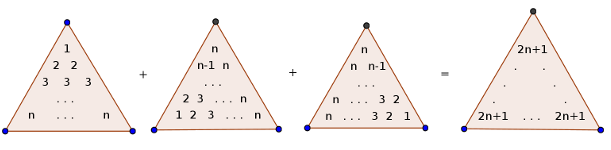
\includegraphics[width=\textwidth]{figure/triangle-proof.png}
\end{minipage}

На языке формул:
\[
  3S = (2n+1) \cdot (1 + 2 + \ldots + n) = (2n+1)n\frac{n+1}{2}.
\]
\end{solution}
\protect \hypertarget {soln:20.2}{}
\begin{solution}{{20.2}}
  Проекцией вектора $(6, 3, 7, 8, 9, 10, 11)$; $a=6$, $b=5$, $c= 9$;
\end{solution}
\protect \hypertarget {soln:20.3}{}
\begin{solution}{{20.3}}
\end{solution}
\protect \hypertarget {soln:20.4}{}
\begin{solution}{{20.4}}
\begin{enumerate}
\item $\chi^2_d$
\item $d$
\item $2d$
\item $\chi^2_{a+b}$
\end{enumerate}
\end{solution}
\protect \hypertarget {soln:20.5}{}
\begin{solution}{{20.5}}
  $Q= Z_1^2$, зная функцию плотности $Z_1$, $f(z_1) = \frac{1}{\sqrt{2\pi}}\exp(-z_1^2/2)$, находим функцию плотности $Q$;
\end{solution}
\protect \hypertarget {soln:20.6}{}
\begin{solution}{{20.6}}
\end{solution}
\protect \hypertarget {soln:20.7}{}
\begin{solution}{{20.7}}
\end{solution}
\protect \hypertarget {soln:20.8}{}
\begin{solution}{{20.8}}
  $\hat Z = \langle Z, z\rangle \cdot v$;
$\hat Z_i = \langle Z, z\rangle \cdot v_i$;
$\Var(\langle Z, z\rangle)=1$; $\Cov(\hat Z_i, \hat Z_j)=v_i v_j \Var( \langle Z, z\rangle)= v_i v_j$;
\end{solution}
\protect \hypertarget {soln:21.1}{}
\begin{solution}{{21.1}}
  Метод максимального правдоподобия:
  \[
    C_n^{Y_{\text{к}}}C_{n-Y_{\text{к}}}^{Y_{\text{щ}}}a^{Y_{\text{к}}}(2a)^{Y_{\text{щ}}}(1-3a)^{Y_{\text{б}}} \to \max_a
  \]
Решая задачу максимизации Кота Матроскина получаем
\[
\hat a_{КМ} = \frac{Y_{\text{к}} + Y_{\text{щ}}}{3n}
\]

Замечаем, что $Y_{\text{к}} + Y_{\text{щ}} \sim Bin(n, 3a)$. Отсюда $\E(\hat a_{\text{КМ}})=a$, $\Var(\hat a_{\text{КМ}}) = \frac{a(1-3a)}{n}$. Оценка несмещённая и состоятельная.

С точки зрения Пса Шарика, неизвестными являются две вероятности, $a$ и $b$. Он решает задачу максимизации по двум переменным. В результате получается вполне себе интуитивная оценка $\hat a_{\text{ПШ}} = Y_{\text{к}}/n$.

\end{solution}
\protect \hypertarget {soln:21.2}{}
\begin{solution}{{21.2}}
Метод правдоподобия: $\max_n \P(S=80)$. Замечаем, что $S \sim Bin\left(100, p=\frac{100}{n}\right)$. Отсюда, $\hat n_{ML} = 125$.

Метод моментов. Рассмотрим $Y_1$, $Y_2$, \ldots, $Y_n$. Величина $Y_i$ равна 1 если при втором отлове $i$-ый заяц оказался с бантом и 0 иначе.

Метод моментов: $\E(Y_i)|_{n=\hat n}=\bar Y$:
\[
\frac{100}{\hat n_{MM}}=\bar Y
\]
Отсюда
\[
\hat n_{MM} = \frac{100}{\bar Y} = \frac{100^2}{S}
\]
\end{solution}
\protect \hypertarget {soln:21.3}{}
\begin{solution}{{21.3}}
\end{solution}
\protect \hypertarget {soln:21.4}{}
\begin{solution}{{21.4}}
\end{solution}
\protect \hypertarget {soln:21.5}{}
\begin{solution}{{21.5}}
\end{solution}
\protect \hypertarget {soln:22.1}{}
\begin{solution}{{22.1}}
  $\hat{\theta}_{ML}=0.25$, $\hat{\theta}_{MM}=0.2$
  $\hat{\theta}_{MM}=\frac{2{,}4-\bar{X}}{7}$
\end{solution}
\protect \hypertarget {soln:22.2}{}
\begin{solution}{{22.2}}
$\hat{a}=\ln(Y_{1})$, $\hat{b}=\ln(Y_{2})-\ln(Y_{1})$
\end{solution}
\protect \hypertarget {soln:22.3}{}
\begin{solution}{{22.3}}
\end{solution}
\protect \hypertarget {soln:22.4}{}
\begin{solution}{{22.4}}
\end{solution}
\protect \hypertarget {soln:22.5}{}
\begin{solution}{{22.5}}
\end{solution}
\protect \hypertarget {soln:22.6}{}
\begin{solution}{{22.6}}
$\hat{a}_{ml}=\sum X_i^2/2n$, $\hat{a}_{mm}=\bar{X}$.
\end{solution}
\protect \hypertarget {soln:22.7}{}
\begin{solution}{{22.7}}
\end{solution}
\protect \hypertarget {soln:22.8}{}
\begin{solution}{{22.8}}
\end{solution}
\protect \hypertarget {soln:22.9}{}
\begin{solution}{{22.9}}
\end{solution}
\protect \hypertarget {soln:22.10}{}
\begin{solution}{{22.10}}
\end{solution}
\protect \hypertarget {soln:22.11}{}
\begin{solution}{{22.11}}
\end{solution}
\protect \hypertarget {soln:22.12}{}
\begin{solution}{{22.12}}
\end{solution}
\protect \hypertarget {soln:22.13}{}
\begin{solution}{{22.13}}
\end{solution}
\protect \hypertarget {soln:22.14}{}
\begin{solution}{{22.14}}
\end{solution}
\protect \hypertarget {soln:22.15}{}
\begin{solution}{{22.15}}
\end{solution}
\protect \hypertarget {soln:22.16}{}
\begin{solution}{{22.16}}
\end{solution}
\protect \hypertarget {soln:22.17}{}
\begin{solution}{{22.17}}
\end{solution}
\protect \hypertarget {soln:22.18}{}
\begin{solution}{{22.18}}
\end{solution}
\protect \hypertarget {soln:22.19}{}
\begin{solution}{{22.19}}
\end{solution}
\protect \hypertarget {soln:22.20}{}
\begin{solution}{{22.20}}
\end{solution}
\protect \hypertarget {soln:22.21}{}
\begin{solution}{{22.21}}
\begin{enumerate}
\item $\E(X_i) = a$, $\E(|X_i|) = 5a/4$
\item $\hat a = 11/30$
\item $\hat a = 26/75$
\item $\hat{a}_{GMM} = 108/325$
\item $\begin{pmatrix}
37 & -44 \\
-44 & 64
\end{pmatrix}$
\end{enumerate}
\end{solution}
\protect \hypertarget {soln:22.22}{}
\begin{solution}{{22.22}}
\end{solution}
\protect \hypertarget {soln:22.23}{}
\begin{solution}{{22.23}}
  $\plim_{n\to\infty} \hat\alpha_{ML}(n) = 0$, не является состоятельной
\end{solution}
\protect \hypertarget {soln:22.24}{}
\begin{solution}{{22.24}}

\end{solution}
\protect \hypertarget {soln:23.1}{}
\begin{solution}{{23.1}}
    \begin{enumerate}
      \item $c=1/n$, да
      \item $c=1/(n+\sigma^2/\mu^2)$, нет, так как $\mu$ и $\sigma$ неизвестны
      \item $\lambda=0$ и $\lambda=\sigma^2/\mu^2$
    \end{enumerate}
  
\end{solution}
\protect \hypertarget {soln:23.2}{}
\begin{solution}{{23.2}}
    \begin{enumerate}
    \item несмещённая, состоятельная, линейная, неэффективная
    \item несмещённая, состоятельная, линейная, неэффективная
    \item несмещённая, несостоятельная, линейная, неэффективная
    \item смещённая, состоятельная, линейная
    \item смещённая, состоятельная, нелинейная
    \item несмещённая, состоятельная, линейная, неэффективная
    \item несмещённая, состоятельная, линейная, эффективная
    \item смещённая, несостоятельная, линейная
    \item смещённая, несостоятельная, нелинейная
    \item несмещённая, состоятельная, линейная, неэффективная
    \end{enumerate}
  
\end{solution}
\protect \hypertarget {soln:23.3}{}
\begin{solution}{{23.3}}
\begin{enumerate}
\item $\hat\theta_{ML} = \max\{ Y_1, Y_2, \ldots, Y_n\}$.
\item Все $Y_i$ меньше $\theta$, значит и $\hat\theta$ всегда меньше $\theta$, значит смещённая.
\item $F_{\hat\theta}(t) = \P(\hat\theta \leq t) = \P(Y_1 \leq t, Y_2 \leq t, \ldots) = (\P(Y_1 \leq t))^n$, $\P(Y_1 \leq t) = t^5/\theta^5$, $f_{\hat\theta}(t) = dF_{\hat\theta}(t)/dt = \frac{5n t^{5n-1}}{\theta^{5n}}$.
\item $\E(\hat\theta) = \frac{5n}{5n+1}\theta$.
\item $\hat\theta_{unbiased} = \frac{5n+1}{5n}\hat\theta$.
\end{enumerate}
\end{solution}
\protect \hypertarget {soln:23.4}{}
\begin{solution}{{23.4}}
\begin{enumerate}
  \item $\hat p$ несмещённая
  \item $\sigma^2 = n p(1-p)$.
  \item $\E(\hat\sigma^2) = (n-1)p(1-p)$, смещённая, $\hat\sigma^2_{unbiased} = \frac{n}{n-1} \hat\sigma^2$.
\end{enumerate}
\end{solution}
\protect \hypertarget {soln:23.5}{}
\begin{solution}{{23.5}}

\end{solution}
\protect \hypertarget {soln:23.6}{}
\begin{solution}{{23.6}}

\end{solution}
\protect \hypertarget {soln:23.7}{}
\begin{solution}{{23.7}}

\end{solution}
\protect \hypertarget {soln:23.8}{}
\begin{solution}{{23.8}}

\end{solution}
\protect \hypertarget {soln:23.9}{}
\begin{solution}{{23.9}}

\end{solution}
\protect \hypertarget {soln:23.10}{}
\begin{solution}{{23.10}}

\end{solution}
\protect \hypertarget {soln:23.11}{}
\begin{solution}{{23.11}}

\end{solution}
\protect \hypertarget {soln:23.12}{}
\begin{solution}{{23.12}}
  Закон распределения $X$ также экспоненциальный, но с другим $\lambda$. Честно находим $\E(X)=\theta/20$, отсюда
  $\hat\theta_{unbiased} = 20X$.
\end{solution}
\protect \hypertarget {soln:23.13}{}
\begin{solution}{{23.13}}

\end{solution}
\protect \hypertarget {soln:23.14}{}
\begin{solution}{{23.14}}
Обе оценки несмещённые, состоятельные. Более эффективна $\hat{\beta}_{2}=\frac{\sum{x_{i}Y_{i}}}{\sum x_{i}^{2}}$.
\end{solution}
\protect \hypertarget {soln:23.15}{}
\begin{solution}{{23.15}}

\end{solution}
\protect \hypertarget {soln:24.1}{}
\begin{solution}{{24.1}}
  $\frac{1}{1.8} - \frac{1}{2.2}$, $[0;10X]$.
\end{solution}
\protect \hypertarget {soln:24.2}{}
\begin{solution}{{24.2}}
\end{solution}
\protect \hypertarget {soln:24.3}{}
\begin{solution}{{24.3}}
\end{solution}
\protect \hypertarget {soln:24.4}{}
\begin{solution}{{24.4}}
\end{solution}
\protect \hypertarget {soln:24.5}{}
\begin{solution}{{24.5}}
\end{solution}
\protect \hypertarget {soln:24.6}{}
\begin{solution}{{24.6}}
Важна при обоих доверительных интервалах. Без предпосылки о нормальности интервал для дисперсии по данным формулам нельзя построить даже при больших $n$. При больших $n$ можно отказаться от предпосылки о нормальности при построении интервала для $\mu$.
\end{solution}
\protect \hypertarget {soln:24.7}{}
\begin{solution}{{24.7}}
\end{solution}
\protect \hypertarget {soln:25.1}{}
\begin{solution}{{25.1}}
к 1/2
\end{solution}
\protect \hypertarget {soln:25.2}{}
\begin{solution}{{25.2}}
  равномерно, $\alpha=0.05$; нет, он резко увеличивает ошибку второго рода
\end{solution}
\protect \hypertarget {soln:25.3}{}
\begin{solution}{{25.3}}
  $\alpha = 1/8$, $\beta = 9/32$
\end{solution}
\protect \hypertarget {soln:25.4}{}
\begin{solution}{{25.4}}
  $\alpha = \P(\cN(0;1) > -0.35) \approx 0.64$, $\beta = \P(\cN(0;1) \leq -1.76) \approx 0.04$.
\end{solution}
\protect \hypertarget {soln:25.5}{}
\begin{solution}{{25.5}}
\end{solution}
\protect \hypertarget {soln:25.6}{}
\begin{solution}{{25.6}}
\end{solution}
\protect \hypertarget {soln:25.7}{}
\begin{solution}{{25.7}}

\end{solution}
\protect \hypertarget {soln:25.8}{}
\begin{solution}{{25.8}}
Критерий Неймана-Пирсона сводится к сравнению $\bar X$ с порогом. При верной $H_0$ величина $\bar X$ распределена $\cN(0; \frac{4}{n})$.
Отсюда искомый критерий имеет вид:
Если $\bar X  \geqslant 0.825$, то гипотеза ${H_0}$ отвергается в пользу гипотезы ${H_a}$.
\end{solution}
\protect \hypertarget {soln:25.9}{}
\begin{solution}{{25.9}}
  Упрощая неравенство из леммы Неймана-Пирсона, получаем критерий: если $X_1\cdot X_2 >t$, то $H_0$ отвергается. Величину $t$ находим из уравнения
\[
\int_0^t (1 - t/x) \, dx = 0.05
\]
\end{solution}
\protect \hypertarget {soln:25.10}{}
\begin{solution}{{25.10}}

\end{solution}
\protect \hypertarget {soln:25.11}{}
\begin{solution}{{25.11}}
\end{solution}
\protect \hypertarget {soln:26.1}{}
\begin{solution}{{26.1}}
При $p_N$ заданном в $H_0$ критерий Пирсона имеет хи-квадрат распределение с двумя степенями свободы.
При оцениваемом $p_N$ критерий Пирсона имеет хи-квадрат распределение с одной степенью свободы.

\url{https://ru.wikipedia.org/wiki/Закон_Харди_—_Вайнберга}
  
\end{solution}
\protect \hypertarget {soln:27.1}{}
\begin{solution}{{27.1}}
$\E(Ay)=A\E(y)$, $\Var(Ay)=A\Var(y)A^T$
\end{solution}
\protect \hypertarget {soln:27.2}{}
\begin{solution}{{27.2}}

\end{solution}
\protect \hypertarget {soln:27.3}{}
\begin{solution}{{27.3}}

\end{solution}
\protect \hypertarget {soln:27.4}{}
\begin{solution}{{27.4}}

\end{solution}
\protect \hypertarget {soln:27.5}{}
\begin{solution}{{27.5}}

\end{solution}
\protect \hypertarget {soln:27.6}{}
\begin{solution}{{27.6}}

\end{solution}
\protect \hypertarget {soln:28.1}{}
\begin{solution}{{28.1}}
Вычтем $2x^2 + 2y^2 + 2z^2 + 2w^2$. Получим, что оптимальное $x=0$. Далее, $z=0$, $y=0$. В итоге $w=1$ или $w=-1$.
\end{solution}
\protect \hypertarget {soln:28.2}{}
\begin{solution}{{28.2}}
\end{solution}
\protect \hypertarget {soln:28.3}{}
\begin{solution}{{28.3}}
\end{solution}
\protect \hypertarget {soln:28.4}{}
\begin{solution}{{28.4}}
\end{solution}
\protect \hypertarget {soln:28.5}{}
\begin{solution}{{28.5}}
$(5+4+1)=10$; длины — $\sqrt{5}\cdot\sqrt{99}$, $\sqrt{4}\cdot\sqrt{99}$, $\sqrt{1}\cdot\sqrt{99}$; выборочные дисперсии — $5$, $4$, $1$; $(5+4)/10=0.9$.
\end{solution}
\protect \hypertarget {soln:28.6}{}
\begin{solution}{{28.6}}
\end{solution}
\protect \hypertarget {soln:29.1}{}
\begin{solution}{{29.1}}
  
\end{solution}
\protect \hypertarget {soln:29.2}{}
\begin{solution}{{29.2}}
  
\end{solution}
\protect \hypertarget {soln:29.3}{}
\begin{solution}{{29.3}}
  
\end{solution}
\protect \hypertarget {soln:30.1}{}
\begin{solution}{{30.1}}
$C_{20}^2\cdot 18$.
\end{solution}
\protect \hypertarget {soln:30.2}{}
\begin{solution}{{30.2}}
  $1+x+x^2+x^3+x^4=(1-x^5)/(1-x)$
  $1+x+x^2+x^3+\ldots = 1/(1-x)$
  $(1+x)^4$
\end{solution}
\protect \hypertarget {soln:30.3}{}
\begin{solution}{{30.3}}
\end{solution}
\protect \hypertarget {soln:30.4}{}
\begin{solution}{{30.4}}
\end{solution}
\protect \hypertarget {soln:30.5}{}
\begin{solution}{{30.5}}
  0 с вероятностью 1/4 и 1 с вероятностью 3/4
\end{solution}
\protect \hypertarget {soln:30.6}{}
\begin{solution}{{30.6}}
  да, сможет!
\end{solution}
\protect \hypertarget {soln:30.7}{}
\begin{solution}{{30.7}}
$F_n = F_{n-1} + F_{n-2}$.
Запишем разложения для $g(x)$, $xg(x)$ и $x^2 g(x)$ друг под другом. Вычитаем. Получаем, что $g(x) = x/(1-x-x^2)$.

Указанная дробь — это и есть производящая функция при маленьком $x$.

Производящая функция представима в виде суммы:
\[
g(x) = \frac{1}{\sqrt{5}}\left( \frac{a}{x+a} - \frac{b}{x+b}  \right),
\]
где $a=(1-\sqrt{5})/2$, $b=(1+\sqrt{5})/2$.
\end{solution}
\protect \hypertarget {soln:30.8}{}
\begin{solution}{{30.8}}
Замечаем, что $h_2(t)=h_1(t)\cdot h_1(t)$. После первого шага:
\[
h_1(t) = 0.7t + 0.3th^2_1(t)
\]
\end{solution}
\protect \hypertarget {soln:30.9}{}
\begin{solution}{{30.9}}

\end{solution}
\protect \hypertarget {soln:31.1}{}
\begin{solution}{{31.1}}
\end{solution}
\protect \hypertarget {soln:31.2}{}
\begin{solution}{{31.2}}
\end{solution}
\protect \hypertarget {soln:32.1}{}
\begin{solution}{{32.1}}
  Если величина $X$ равновероятно принимает $k$ значений, то спутанность равна $k$. У равномерной на $[0;a]$ спутанность равна $a$.
\end{solution}
\protect \hypertarget {soln:32.2}{}
\begin{solution}{{32.2}}
\end{solution}
\protect \hypertarget {soln:32.3}{}
\begin{solution}{{32.3}}
\end{solution}
\protect \hypertarget {soln:32.4}{}
\begin{solution}{{32.4}}
\end{solution}
\protect \hypertarget {soln:32.5}{}
\begin{solution}{{32.5}}
\end{solution}
